\documentclass{article}

% Language setting
% Replace `english' with e.g. `spanish' to change the document language
\usepackage[english]{babel}

% Set page size and margins
% Replace `letterpaper' with`a4paper' for UK/EU standard size
\usepackage[letterpaper,top=2cm,bottom=2cm,left=3cm,right=3cm,marginparwidth=1.75cm]{geometry}

% Useful packages
\usepackage{amsmath}
\usepackage{graphicx}
\usepackage[colorlinks=true, allcolors=blue]{hyperref}

\title{GUFI: A Common User's Guide}
\author{Braeden Slade}

\begin{document}
\maketitle

\section{Introduction}
Over the years, the amount of data we store and use has grown exponentially to the point that petabytes of storage is not uncommon. What used to be a simple task of accessing and sorting through information has been compounded into an arduous task with the size and scale of super-computing data centers. Being able to query data effectively, while also taking into account permissions becomes paramount into accomplishing daily tasks. This is what the Grand Unified File Index(GUFI) tool aims to accomplish. 

\subsection{Background}
This is accomplished by recreating the tree structure via indexing. Each directory contains an SQL database file that stores the metadata of the files as well as summary information for that directory and optionally summary information for the entire tree below that directory. 

\begin{figure} [h]
\centering
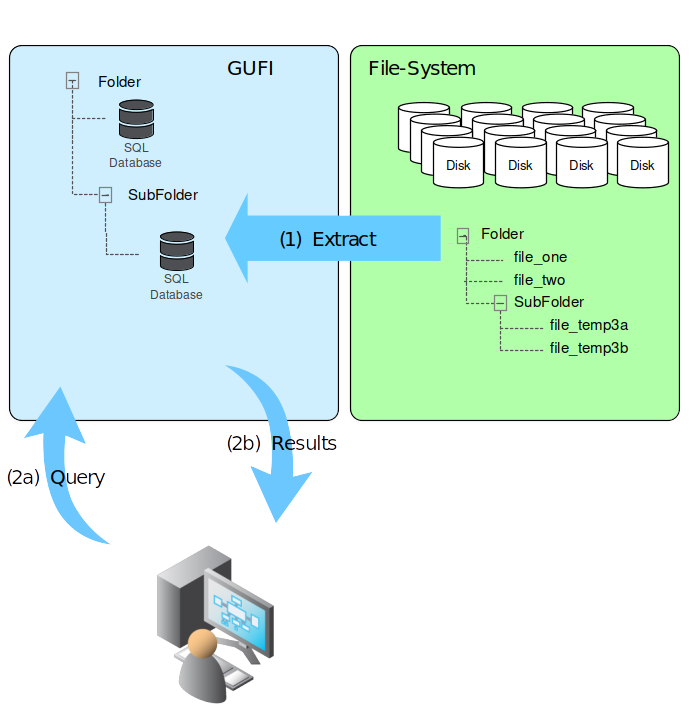
\includegraphics[width=0.5\textwidth]{gufi_structure.png}
\caption{\label{fig:gufi\_structure}Layout and user interaction with GUFI}
\end{figure}

\clearpage

\section{gufi\_find}
gufi\_find is a high level script that allows for users to search through a GUFI index and provide a variety of specifications/arguments. The user may provide as many, or as few specifications/arguments as they desire to find the file(s) they want. A comprehensive list of all available arguments is listed below 

\begin{table} [h]
\centering
\begin{tabular}{l}
Arguments available \\\hline
--help\\
--maxdepth \textless levels\textgreater\\
--mindepth \textless levels\textgreater\\
--version\\
--amin \textless n\textgreater\\
--atime \textless n\textgreater\\
--cmin \textless n\textgreater\\
--ctime \textless n\textgreater\\
--empty\\
--executable\\
--false\\
--gid \textless n\textgreater\\
--group \textless gname\textgreater\\
--iname \textless pattern\textgreater\\ 
--inum \textless n\textgreater\\
--links \textless n \textgreater\\
--lname \textless pattern\textgreater\\
--mmin \textless n\textgreater\\
--mtime \textless n\textgreater\\
--name \textless pattern\textgreater\\
--newer \textless file\textgreater\\
--path \textless pattern\textgreater\\
--reabable\\
--samefile\\
--size \textless n\textgreater\\
--true\\
--type \textless c\textgreater\\
--uid \textless n\textgreater\\
--user \textless name\textgreater\\
--writable\\
--fprint \textless file\textgreater\\
--printf \textless format\textgreater\\
--delim \textless c \textgreater\\
--num-results \textless n\textgreater\\
--smallest\\
--largest\\
--output-buffer \textless bytes\textgreater\\
--inmemory-name \textless name \textgreater
\end{tabular}
\caption{\label{tab:widgets}List of available arguments}
\end{table}

\clearpage

\section{gufi\_ls}
gufi\_ls functions like the POISX command ls. As with gufi\_find, there are a multitude of options available listed below

\subsection{Flags and Functionality}
\begin{table} [h]
\centering
\begin{tabular}{l|r}
Flags & Functionality\\\hline
--help & displays help menu\\
-v, --version & show program's version number and exit \\
-a, --all & do not ignore entries ending with .\\
-A, --almost-all & do not list implied . and .. \\
--block-size \textless block\_size\textgreater & with -l, scale sizes by block\_size when printing them \\
-B, --ignore-backups & do not list implied entries ending with ~\\
-G, --no-group & in a long listing, don't print group names\\
-i, --inode & print the index number of each file\\
-l & used a long listing format\\
-r, --reverse & reverse order while sorting\\
-R, --recursive & list sub-directories recursively\\
-s, --size & print the allocated size of each file in blocks\\
-S & sort by file size, largest first \\
--time-style \textless TIME\_STYLE\textgreater & time/date format with -l\\
-t & sort by modification time, newest first\\
-U & do not sort; list entries in directory order\\
--delim \textless c\textgreater & delimeter separating output columns\\ 
--in-memory-name \textless name\textgreater & Name of in-memory database when -R is used\\
--nlink-width \textless chars\textgreater & Width of nlink column\\
--size-width \textless chars\textgreater & Width of size column\\
--user-width \textless chars\textgreater & Width of user column\\
--group-width \textless chars\textgreater & width of group column
\end{tabular}
\caption{\label{tab:widgets}Flags and Functionality}
\end{table}

\clearpage

\section{gufi\_stats}
gufi\_stats is used to analyze a tree and return generic statistics the user requests for

\subsection{Stats list}
\begin{table} [h]
\centering
\begin{tabular}{l}
Stats\\\hline
depth \\
filesize \\
filecount \\
linkcount \\
dircount \\
leaf-dirs \\
leaf-depth \\
leaf-files \\
leaf-links \\
total-filesize \\
total-filecount \\
total-linkcount \\
total-dircount \\
total-leaf-files \\
total-leaf-links \\
files-per-level \\ 
links-per-level \\
dirs-per-level \\
average-leaf-files \\
average-leaf-links \\ 
median-leaf-files \\
duplicate-names
\end{tabular}
\caption{\label{tab:widgets}List of available stats}
\end{table}

\begin{table} [h]
\centering
\begin{tabular}{l|r}
Optional Flags & Functionality\\\hline
--help & displays help menu\\ 
--version, -v & display program's version number and exits \\
--recursive, -r & run command recursively \\
--cumulative -c & return cumulative values \\
--order \textless order\textgreater & sort output (if applicable)\\
--delim \textless c\textgreater & delimeter separating output columns\\
--num-results \textless n\textgreater & first n results \\
--uid \textless u\textgreater, --user \textless u\textgreater & restrict to user \\
--in-memory-name \textless name\textgreater & Name of in-memory database when -R is used
\end{tabular}
\caption{\label{tab:widgets}Flags and Functionality}
\end{table}

\subsection{Structure and example call}
gufi\_stats [optional flags] [stat] \\
EX: ./gufi\_stats --delim + total-filecount
\end{document}